
\documentclass[10pt,conference,a4paper]{IEEEtran}
     
%%% PAQUETES  %%%
%%% PAQUETES  %%%

%%% Soporte extendido de colores
\usepackage{xcolor}
    % Definiciones colores extra
    %% Ref: http://latexcolor.com/
    \definecolor{coolblack}{rgb}{0.0, 0.18, 0.39}
    \definecolor{dimgray}{rgb}{0.41, 0.41, 0.41}

%%% Paquete para poner hipervinculos más finos \href
\PassOptionsToPackage{hyphens}{url}
\usepackage{hyperref}

   %Colores personalizados
    \hypersetup{
        colorlinks=true,
        linkcolor=black,
        filecolor=black,
        %%% Necesita su propia definicion de color
        citecolor=dimgray,
        urlcolor=coolblack,
    }

%%% Formato y tipografía de URL, direcciones de correo...
\usepackage{url}
    \def\UrlFont{\rmfamily}

%%% Usados por graficas de barras
\usepackage{textcomp}
\usepackage{tikz}
\usepackage{pgfplots}
\usepackage{pgfplotstable} 
\usepackage{csvsimple}% Generates table from .csv
\pgfplotsset{compat=1.7}
\usepackage{subcaption}
\usepgfplotslibrary{groupplots}

% PGFPlots Settings
\pgfplotsset{
SmallBarPlot/.style={
    font=\footnotesize,
    ybar,
    width=\linewidth,
    ymin=0,
    xtick=data,
    xticklabel style={text width=1.5cm, rotate=90, align=center}
},
BlueBars/.style={fill=blue!20, bar width=0.25},
RedBars/.style={fill=red!20, bar width=0.25},
GreenBars/.style={fill=green!20, bar width=0.25}
}

%% Para incluir en el texto o en el pie de la figura la leyenda con colores.
\DeclareRobustCommand\legendbox[1]{(\textcolor{#1}{#1 bars}~\begin{tikzpicture}[x=0.2cm, y=0.2cm] \draw [color=black, fill=#1!20] (0,0) -- (0,1) -- (0.6,1) -- (0.6,0) -- (0, 0); \end{tikzpicture})}

\usepackage{booktabs} % usado en tablas generadas con JASP


%%%%%%%%%%%%%%%%%%%%%%%%%%%%%%% HEREDADOS JNIC %%%%%%%%%%%%%%%%%%%%%%%%%%%%%%%

%%% TODO NOTES y definición 2cm de margen para que no se solapen añadido colores comentarios
 \setlength {\marginparwidth }{2cm} 
 \usepackage{todonotes}
 \usepackage[normalem]{ulem}

%%% Paquete para comentarios
\usepackage{verbatim}

%%% Tildes y demás caracteres en castellano...
%\usepackage[latin1]{inputenc}
% o bien
\usepackage[utf8]{inputenc}

%%% Fuente Times...
\usepackage{times}

%%% Figuras en formato .png, .ps, pdf o eps
\usepackage{graphicx}
%%\usepackage{subfigure}
\DeclareGraphicsExtensions{.png,.eps,.ps,.pdf}

%%% Soporte graficos svg
\usepackage{svg}

%%% Sección para definir explícitamente la separación de sílabas al final de una línea:
\hyphenation{si-guien-do}

%%% Secciones etc. en castellano
%\usepackage[spanish,es-tabla]{babel}

%%% Secciones etc. en Ingles
\usepackage[english]{babel}


%%% Paquete para usar simbolos y scripts de dibujado
\usepackage{tikz}
\def\checkmark{\tikz\fill[scale=0.4](0,.35) -- (.25,0) -- (1,.7) -- (.25,.15) -- cycle;} 
\usetikzlibrary{shapes,arrows}

% Define Block styles
\tikzstyle{decisionBL} = [diamond, draw, fill=blue!20,text width=10em, text badly centered, node distance=3cm, inner sep=0pt]
\tikzstyle{blockBL} = [rectangle, draw, fill=blue!20,text width=9em, text centered, rounded corners, minimum height=4em]
\tikzstyle{blockYL} = [rectangle, draw, fill=yellow!20, text width=9em, text centered, rounded corners, minimum height=4em]
\tikzstyle{blockGR} = [rectangle, draw, fill=green!20, text width=9em, text centered, rounded corners, minimum height=4em]
\tikzstyle{blockRD} = [rectangle, draw, fill=red!20, text width=9em, text centered, rounded corners, minimum height=4em]
\tikzstyle{blockWH} = [rectangle, draw, fill=white!20, text width=9em, text centered, rounded corners, minimum height=4em]
\tikzstyle{line} = [draw, -latex']
\tikzstyle{cloud} = [draw, ellipse,fill=red!20, node distance=4.5cm,minimum height=4em]

%%% Para usar ficheros tex de infografias Inkscape
\usepackage{pstricks}
    
%%% COMANDOS  %%%
%%% COMANDOS  %%%

%%% A cursiva  %%%
\newcommand{\cursiva}[1]{\em{#1}}


%%% Fuzzing en bonito  %%%
\newcommand{\fz}{\em fuzzing}

%%% Atajos estilo  %%%

\newcommand{\CLASSINPUTinnersidemargin}{18mm}
\newcommand{\CLASSINPUToutersidemargin}{12mm}
\newcommand{\CLASSINPUTtoptextmargin}{20mm}
\newcommand{\CLASSINPUTbottomtextmargin}{25mm}

\newcommand{\new}[1]{\textcolor{olive}{{#1}}}
%\newcommand{\old}[1]{\textcolor{purple}{{\sout{#1}}}}
\newcommand{\wip}[1]{\textcolor{blue}{{#1}}}
%\newcommand{\checkthis}[1]{\textcolor{orange}{{#1}}}
\newcommand{\diego}[1]{\textcolor{magenta}{{#1}}}
\newcommand{\vmodixit}[1]{\textcolor{teal}{{#1}}}

\newcommand{\old}[1]{\textcolor{purple}{{\sout{#1}}}}
\newcommand{\camino}[1]{\textcolor{olive}{{#1}}}
\newcommand{\fjrodl}[1]{\textcolor{blue}{{#1}}}
\newcommand{\checkthis}[1]{\textcolor{orange}{{#1}}}

%%% Entornos  %%%
\newcounter{definicion}
\newenvironment{definicion}[1]{%
    \refstepcounter{definicion}\par\medskip%
    \noindent \textbf{Definición~\thedefinicion. #1}.\ %
}{\medskip}

%%%% Soporte para el logo de ORCID
%\newcommand{\orcid}[1]{\href{https://orcid.org/#1}{\textcolor[HTML]{A6CE39}{\aiOrcid}}}


  
\begin{document}
 
%%% Título
\title{HOUSE: Marco de trabajo modular de arquitectura escalable y desacoplada para el uso de técnicas de {\fz} en HPC}

%%% Autores
%\author{\IEEEauthorblockN{Francisco Borja Garnelo Del Río, Francisco J. Rodríguez Lera, Gonzalo Esteban Costales, \\ %Camino Fernández Llamas, Vicente Matellán Olivera}
%\IEEEauthorblockA{Universidad de León - 
%Campus de Vegazana s/n, 24071 León (Spain)\\
%infbgd01@estudiantes.unileon.es, \{fjrodl, gestc, cferll, vmato\}@unileon.es
%}}

% Depepende de \usepackage{svg}
\newcommand{\orcid}[1]{\href{https://orcid.org/#1}{
\includegraphics[width=8pt]{figures/data/orcid_logo.png}}}


\author{\IEEEauthorblockN{Francisco Borja Garnelo Del Río \orcid{0000-0002-8935-0669}, Francisco J. Rodríguez Lera \orcid{0000-0002-8400-7079}, Gonzalo Esteban Costales \orcid{0000-0003-3645-164X}, \\ Camino Fernández Llamas \orcid{0000-0002-8705-4786}, Vicente Matellán Olivera \orcid{0000-0001-7844-9658}}
\IEEEauthorblockA{Universidad de León - 
Campus de Vegazana s/n, 24071 León (Spain)\\
infbgd01@estudiantes.unileon.es, \{fjrodl, gestc, cferll, vmato\}@unileon.es
}}


%\author{
%  Francisco Borja Garnelo Del Río \orcid{0000-0002-8935-0669}, \and
%  Francisco J. Rodríguez Lera \orcid{0000-0002-8400-7079},\and
%  Gonzalo Esteban Costales \orcid{0000-0003-3645-164X},\and
% Camino Fernández Llamas \orcid{0000-0002-8705-4786},\and
%  Vicente Matellán Olivera \orcid{0000-0001-7844-9658}
%  }

\maketitle

%%% Resumen del paper en base a objetivos
\begin{abstract}

%%%%%%%%%%%%%%%%%%%%%%%%%%%%%%%%%%%%%%%%%%%%%%%%%%%%%%%%%%%%%%%%%%%%%

El {\fz} es una técnica de prueba automatizada que hace uso de mutaciones de entradas para ejecutar el software utilizando estas a fin de observar los valores de retorno y el estado externo del sistema; todo ello para identificar comportamientos no esperados.
Por su simpleza y fácil automatización inicial, el {\fz} es una de las técnicas más populares para identificar vulnerabilidades en software en el mundo real. El uso de técnicas de {\fz} como parte del desarrollo de software en grandes compañías ha acelerado la evolución de las técnicas y mejorado las herramientas, como contrapartida muchos proyectos quedan huérfanos de sus desarrolladores originales, al ser captados por estas empresas y todas aquellas características con potencial uso comercial, son restringidas al ámbito privado o son dependientes de nubes propietarias. Esto supone una barrera inicial para nuevos desarrollos, una posible dependencia tecnológica de terceros y problemas de confidencialidad de los datos para adoptar modelos seguros de desarrollo o realizar investigaciones. Las investigaciones sobre {\fz} y las nuevas herramientas tienen en común partir desde cero o una base teórica y focalizarse en una característica o funcionalidad. 
Por todo lo anterior resulta valioso desarrollar un marco de trabajo común que de coherencia y continuidad de forma global abordando el {\fz} como un flujo con distintas fases, organizando todos los procesos implicados, incluyendo también aquellos con relación directa, de forma modular, abierta y agnóstica a las herramientas y técnicas.
Con ello se potencia la reutilización y se elimina la dependencia a herramientas o casos de uso, a la vez que permiten sinergias con otros enfoques de seguridad en el software. El uso de una arquitectura desacoplada y escalable permite la distribución y paralelización de trabajos. Esta arquitectura es ideal para entornos de computación de alto rendimiento en adelante HPC ( high-performance computing por su traducción al inglés) 
%HPC\footnote{\textbf{HPC} High-Performance Computing, computación de alto rendimiento o supercomputación.} 
o basados en cargas de trabajo. El código fuente y la documentación empleada para la prueba de concepto se encuentra disponible públicamente en GitHub.

\end{abstract}


%%% Palabras clave
\begin{IEEEkeywords}
Desarrollo seguro, marco de trabajo, {\fz}, análisis de datos, adaptación de código, HPC, seguridad del software, automatización pruebas software, SDL, AFL++, Slurm
\end{IEEEkeywords}

%%% TODO %%%% Resto plantilla JNIC completar o quitar
% {\bf Tipo de contribución:} {\it Investigación original (límite 8 páginas)}

%%% Consejos generales 
\section{Introducción}

%%%%%%%%%%%%%%%%%%%%%%%%%%%%%%%%%%%%%%%%%%%%%%%%%%%%%%%%%%%%%%%%%%%%%
% Como te he puesto en el comentario, esta sección es muy amplia.
% Creo que simplemente habría que reorganizarla siguiendo una
% estructura parecida a la del abstract; moviendo algunas cosas a
% otras secciones (como la del background). Concretamente, la
% introducción sería algo del estilo:
%
%   1. Contexto, motivación/justificación del trabajo. Lo mismo que
%   en el abstract, pero ampliado algo más, de este modo tendrías 2
%   ó 3 párrafos (uno para el contexto y uno/dos para la
%   motivación/justificación).
%   2. Objetivo del trabajo y solución. 1 ó 2 párrafos en los que
%   expliques cuál es el objetivo del paper, presentar HOUSE y cuáles
%   son sus principales características.
%   3. Estructura del artículo. 1 párrafo en el que digas que el
%   artículo tiene tantas secciones y, expliques con una frase de qué
%   va cada sección
%%%%%%%%%%%%%%%%%%%%%%%%%%%%%%%%%%%%%%%%%%%%%%%%%%%%%%%%%%%%%%%%%%%%%



%%%% Contexto histórico general

El {\fz}~\cite{contexto_fuzzing} es la automatización de generación y prueba de entradas malformadas en el software con el fin de encontrar comportamientos no esperados en el mismo, habitualmente \textit{crashes}%
\footnote{\textbf{\textit{crash}}~\cite{IEEE_SW_standar}
Fallo repentino y completo de un sistema o componente informático.
}. %
Este término se usó por primera vez en un estudio de la seguridad de UNIX en la década de 1990~\cite{inicio_fuzzing,continuacion_fuzzing}.

Hace poco más de una década, las herramientas de {\fz} eran poco más que generadores de ruido aleatorio. En la actualidad hay nuevas técnicas capaces de entender en mayor medida la semántica y los flujos de ejecución del software de forma automatizada. Algunos ejemplos son la generación de firmas~\cite{fuzz_evo-tec-firma}, la ejecución simbólica dinámica~\cite{fuzz_evo-tec-ejec_simbolica_dina}, las pruebas de complejidad~\cite{fuzz_evo-tec-complex}, la generación de casos de prueba basados en gramáticas~\cite{fuzz_evo-tec-gem_tc_grama} y las pruebas de comportamiento~\cite{fuzz_evo-tec-comportamiento}. 

Las últimas investigaciones han avanzado mucho en las capacidades de generación de entradas y en el análisis de las estructuras internas del software; ambas con el fin de evolucionar características o funcionalidades de las herramientas de {\fz}. Gran parte del éxito de estas investigaciones ha venido de la mano de aplicar los últimos avances en el análisis de datos~\cite{anal_datos} y algoritmos de aprendizaje automatizado~\cite{aprend_auto} o de su uso específico para la búsqueda de vulnerabilidades%
\footnote{\textbf{Vulnerabilidad}~\cite{ENISA_risk_security_ref}
La existencia de una debilidad, diseño o error de implementación que puede llevar a un evento inesperado e indeseable que comprometa la seguridad del sistema informático, red, aplicación o protocolo involucrados.
}
de seguridad~\cite{fuzzing_V-Fuzz}. Como respuesta a su uso como herramienta de búsqueda de vulnerabilidades, también están surgiendo técnicas \textit{antifuzzing}~\cite{fuzzing_antifuzz}.

Respecto a su uso a gran escala fuera del ámbito privado, se han realizado experimentos de su uso en HPC~\cite{HPC_fuzzing} y es posible replicar experimentos parecidos en entornos cloud compatibles con las herramientas y arquitecturas HPC como AWS~\cite{AWS_doc-slurm_plugin}, Azure~\cite{Azure_doc-CycleCloud_slurm} o GCS~\cite{slurm_doc-elastic_aws_gc}. No obstante, el {\fz} no está exento de contratiempos a la hora de su uso o aplicación.

%%% PROBLEMA 1 %%%% Complejidad de modificar una parte sin tener que montar algo complejo para ello (técnicas y herramientas)
La complejidad y la vasta cantidad de información existente sobre el {\fz} es el primer problema que se presenta. Esto suele derivar en que muchos de estos avances son proyectos separados que sólo son implementados como pruebas de concepto de forma aislada, sin ser integrados con otras mejoras, u optimizaciones de forma general, que acaban siendo descontinuados o parcialmente integrados en herramientas \textit{open source}~\cite{fuzz_tool_afl++_paper}.

%%% PROBLEMA 2 %%% Monopolio de las herramientas y confidencialidad de los datos
El segundo problema se debe a la monopolización de las herramientas e investigaciones hacia objetivos comerciales o de uso interno por parte de la industria u organizaciones. Esto es especialmente relevante en aquellos proyectos orientados a utilizar técnicas de {\fz} a gran escala o como parte de un modelo de desarrollo seguro. Tales proyectos presentan serias limitaciones para ser adaptados a distintos entornos diferentes de aquellos para los que fueron creados; ya sea debido a su origen privativo~\cite{HPC_fuzzing_multinode,google_fuzz} o a su enfoque comercial~\cite{microsoft_fuzz,microsoft_tool_azure}.

Esto, en caso de productos comerciales, presenta serias limitaciones de cara a la privacidad dado que implica el acceso al código fuente
%
\footnote{
\textbf{Código fuente}~\cite{IEEE_SW_standar}:
Instrucciones y definiciones de datos del ordenador expresadas en una forma adecuada para su introducción en un ensamblador, compilador u otro traductor. También considerada la versión legible para el ser humano de la lista de instrucciones [programa] que hace que un ordenador realice una tarea.
}
%
y el uso de \textit{Software as a Service} (SaaS) en entornos de nube en alguna de sus modalidades. Respecto a aquellos proyectos de origen privativo, las limitaciones suelen venir por la dificultad de aprendizaje de la solución y por su adaptación a un entorno diferente, con esfuerzos reiterados en cada nueva evolución de la solución original.

La tendencia generalizada a utilizar infraestructuras en la nube, promovidas en gran parte por las mismas organizaciones que derivan el desarrollo de las herramientas al ámbito privado, impactan en una pérdida de autonomía y confidencialidad de los datos. Sirva de ejemplo un proveedor de nube específico~\cite{google_serv} o la toma de decisiones de forma unilateral por el prestador de servicio~\cite{microsoft_srv}.

%%% PROBLEMA 3 %%% Dificultad y especialización, puesta en marcha (Aplicación practica)
Un tercer problema es debido a la dificultad y especialización necesarias para poner en marcha el {\fz} de forma que este aporte valor sin un esfuerzo recurrente y pueda aplicar los resultados de forma efectiva o reutilizar los esfuerzos previos realizados para casos similares.

Realizar pruebas de {\fz} en software es una tarea compleja puesto que requiere preparar~\cite{fuzzing_SOA} el código fuente para facilitar la automatización de entradas. Los protocolos de red o los componentes del núcleo de los sistemas operativos son dos ejemplos de software que necesitan una preparación previa para lograr obtener resultados efectivos.

En los casos donde la entrada de datos presente una complejidad elevada (como por ejemplo reproductores multimedia, intérpretes de lenguajes o protocolos de comunicaciones) implica un proceso previo de generación de entradas~\cite{fuzzing_SOA}. Para ello es necesario preparar las entradas iniciales o semillas utilizando ficheros con estructuras complejas o programables, como pueden ser los documentos XML, JavaScript, etc.

De forma generalizada a todo proceso de {\fz} es necesaria una especialización para el aprovechamiento de los resultados para por ejemplo identificar puntos de mejora de seguridad%
\footnote{\textbf{Seguridad}~\cite{ENISA_risk_security_ref}
Todos los aspectos relacionados con la definición, adquisición y mantenimiento de la confidencialidad de los datos, la integridad, la disponibilidad y la responsabilidad.
}%
 o en la calidad del software.

Estos problemas pueden ser abordados sobre una estructura ordenada y orientada a las fases comunes del {\fz}, con un diseño modular de componentes que permita la reutilización e integración de distintas soluciones. El marco de trabajo HOUSE que se presenta en este trabajo propone una aproximación que permite mantener la confidencialidad del código fuente, garantizando la escalabilidad y funcionamiento independiente de cada uno de sus módulos para evitar esfuerzos recurrentes. Además, facilita la investigación de cada uno de los componentes que forman parte del proceso de {\fz} y la adopción de estas técnicas en proyectos de desarrollo. Esto reduce la barrera inicial y además proporciona una estructura modular consistente que permite simplificar las tareas de integración, preparación-ejecución de pruebas y análisis de resultados. Debido a que brinda una separación funcional, con automatizaciones para su puesta en funcionamiento e integrado en una organización superior preparada para la paralelización y reutilización.

Los principales objetivos de esta investigación son:
\begin{enumerate}
    \item Conocer el estado actual del {\fz} enfocándolo a su uso en entornos computación de alto rendimiento.
    \item Dar una visión global de las actividades previas, los procesos y componentes del fuzzing respecto a las últimas mejoras y las adaptaciones a entornos de computación escalable.
\end{enumerate}




%%% Intro basica

%Así pues, esta investigación persigue sentar las bases teóricas comunes y las prácticas mínimas de un marco de trabajo que permita unificar todos estos esfuerzos. Ello permite reducir el esfuerzo inicial a la hora de poner en marcha un entorno de {\fz} escalable que garantice la confidencialidad de la información. De igual modo, HOUSE facilita, tanto a investigadores como a desarrolladores, el hecho de poder trabajar en un componente o funcionalidad específica o el hecho de incluir aquellas características de seguridad proactiva en el software dentro de su ciclo de desarrollo. Estos aspectos se traducen en una reducción de la carga de trabajo en tareas auxiliares o distintas a las de los objetivos que tengan planificados.

%%% INDICE COTENIDOS, 
%%% Contexto y trabajos relacionados
%%% Marco de trabajo HOUSE
%%%     Flujo de trabajo / Proceso
%%%         Fase_comun
%%%         Fase_prefuzzing
%%%         Fase_fuzzing
%%%         Fase_postfuzzing
%%% Prueba de Concepto
%%%     Descripción del Entorno
%%%     Conclusiones

%%% Desarrollo estructura de contenidos
El resto del artículo se estructura de la siguiente manera. La Sección~\ref{Contexto-trabajos_relacionados} relaciona las distintas disciplinas que convergen o tienen un punto común con el {\fz} (como son el desarrollo seguro de software y la seguridad), así como conceptos clave relacionados o que forman parte de su evolución. La Sección~\ref{Marco_de_trabajo_HOUSE} desarrolla el flujo de trabajo en sus distintas fases atendiendo a los distintos procesos implicados. La Sección~\ref{Prueba_de_concepto} expone la experiencia de uso del marco de trabajo HOUSE en un entorno de supercomputación real. Por último, la Sección~\ref{Conclusiones} detalla las conclusiones del trabajo.
La documentación de uso del Marco de trabajo HOUSE esta disponible el repositorio de GitHub~\cite{HOUSE_ref-github_repo}.

%%% Consejos
\section{Contexto y trabajos relacionados}  \label{Contexto-trabajos_relacionados}

Con la evolución en complejidad y extensión de los sistemas informáticos y de comunicaciones, el software que los gobierna cuenta cada vez con más superficie susceptible de fallos, lo que a su vez supone una mayor dificultad para su búsqueda y prueba.

\subsection{Tipos de pruebas software}

De una forma sencilla podemos reducir los tipos de pruebas realizadas al software en activas o dinámicas y pasivas o estáticas. Activas son aquellas pruebas que implican la ejecución total o parcial del software y las pasivas se centran en analizar el código fuente.

Dentro de las activas o dinámicas, atendiendo a un enfoque puramente de seguridad en el software~\cite{fuzz_ref_sec-qa_sw}, su identificación puede ser proactiva o reactiva.

Según nuestras evidencias, aparentemente no hay alternativas en la literatura al {\fz} desde un enfoque proactivo. El objetivo del {\fz} es identificar por medio de automatizaciones comportamientos no esperados en el software habitualmente en forma de \textit{crashes}. Algunos de estos fallos en el software pueden ser utilizados para comprometer la seguridad del sistema donde este es ejecutado o la información a la que tiene acceso. Debido a la automatización, es necesario acotar las pruebas a un método de entrada de datos específico en el software y limitarlas a un conjunto de funcionalidades que interactúen con las entradas de la manera más determinista posible. Ejemplos de \textit{fuzzers} son herramientas como BFF~\cite{fuzz_tool_BFF}, radamsa~\cite{fuzz_tool_radamsa} o AFL~\cite{fuzz_tool_afl}.

Observando el comportamiento del software en un entorno de producción, es posible identificar de manera reactiva comportamientos no esperados. Estos por ejemplo pueden ser controles basados en contexto, como Security-Enhanced Linux {\em (SELinux)}~\cite{NSA_SELinux} o Application Armor \textit{(AppArmor)}~\cite{Linux_AppArmor}, para distribuciones Linux o soluciones comerciales de seguridad basadas en la monitorización de eventos y protecciones ~\cite{edr_wuml,xdr_ref} siendo las más comunes combinaciones de Endpoint Detection and Response \textit{(EDR)} y Endpoint Protection Platform \textit{(EPP)}.

Existen numerosas herramientas públicas para realizar pruebas automatizadas sobre el software de manera pasiva utilizando su código fuente. Como por ejemplo CodeQL~\cite{src_tool_codeql} centrada en facilitar el análisis semántico del código fuente como si se tratase de consultas a una base de datos, u otras herramientas más tradicionales como los analizadores de código Sonarqube, Yasca o Flawfinder~\cite{src_tool_list-NIST}.

Para realizar análisis más completos es necesario combinar distintos enfoques como el proactivo por medio de {\fz} y el pasivo con herramientas que permitan minimizar o priorizar qué funcionalidades son susceptibles a tener más bugs\footnote{\textbf{Bug}~\cite{IEEE_SW_standar}
Anomalía, defecto, error, excepción o fallo no controlado en un software.
}\footnote{\textbf{Error}~\cite{ISO_stand_computer-data}
La diferencia o discrepancia entre un valor o condición calculado, observado o medido y el valor o condición verdadero, establecido o teóricamente correcto.
}. Este es el caso cuando por complejidad no sea posible realizar pruebas con cobertura completa del alcance o cuando se requieren adaptaciones a medida para permitir la integración de las herramientas de pruebas con el software objetivo. La misma problemática se repite en el caso de querer utilizar infraestructuras de cómputo intensivo como supercomputadores o clusters en la nube~\cite{Azure_doc-CycleCloud_slurm}.

Respecto a los datos utilizados en el proceso, hay algunos componentes de generación de datos de entrada, limpieza de falsos positivos y análisis de resultados, la mayoría teóricos o con una implementación muy dirigida.

Este escenario tan heterogéneo repleto de piezas aisladas dispares o rígidos componentes, hace difícil introducir de forma mantenible en el tiempo y de manera eficiente pruebas de {\fz} en el desarrollo y ralentiza las investigaciones de mejoras de los componentes del proceso.

\subsection{Tipos de fuzzing}

Los tipos de {\fz} se clasifican en función de los detalles de la implementación disponible, estando claramente diferenciados dos tipos por la utilización del código fuente para la realización de las pruebas o el uso de software ya compilado en formato binario ~\cite{fuzz_ref_sec-qa_sw}. Estos dos tipos son el \textit{white-box {\fz}}~\cite{fuzz_ref_WF-auto} y el \textit{black-box {\fz}}~\cite{fuzz_ref_BF-testing} respectivamente.

Entre estos dos tipos se situaría un tercero, el \textit{grey-box {\fz}}~\cite{fuzzing_SOA}, que tiene características de ambos, como es el caso de las pruebas donde se utiliza instrumentación en el código fuente\cite{fuzz_ref_WF-general} y el análisis BVA (\textit{Boundary Value Analysis})~\cite{fuzz_ref_BF-bva} sobre los comportamientos observados en las ejecuciones del binario.

En la actualidad hay múltiples proyectos alrededor del {\fz}, desde el análisis de resultados~\cite{fuzz_analisis-resultados}, creación de conjuntos de datos de entrada de forma automatizada~\cite{fuzzing_IN-gen}, aquellos específicos de tareas internas como optimizaciones~\cite{fuzzing_optimizacion} y creación de algoritmos de prueba~\cite{fuzzing_extensionAFL}. Todos ellos necesitan, para poder ser completados de forma práctica, unas condiciones que en la mayoría de los casos exigen un esfuerzo de creación de un entorno completo de {\fz}. Similar caso sucede a desarrolladores que demanden poder realizar pruebas de calidad o seguridad en su software y quieran mantener la confidencialidad de su código fuente y evitar los esfuerzos de puesta en marcha de un entorno de {\fz} y realizar desde cero su integración o adaptación.

Las pruebas proactivas y activas con fines de calidad centradas en la seguridad ~\cite{fuzz_ref_sec-qa_sw} como el {\fz} están cada vez más presentes en los ciclos de vida de desarrollo de software SDLC (\textit{Software Development Life Cycle)}, siendo parte fundamental de los procesos para la implantación de un modelo de desarrollo seguro SSDLC (\textit{Secure Software Life Cycle)}~\cite{SDL_WOW}.

%--------------------------------------------------------------------

\section{Marco de trabajo HOUSE}
\label{Marco_de_trabajo_HOUSE}

HOUSE es un marco de trabajo con un enfoque funcional que permite organizar todas las actividades necesarias de cara a aplicar técnicas {\fz} sobre un proyecto software. Su nombre hace referencia a la clásica metáfora~\cite{SW_ref_metafora} de describir un proceso como el diseño y construcción de una casa y, en este caso, describe el proceso de desarrollo seguro del software pero desde el punto de vista del {\fz}.

En cuanto a sus características, HOUSE posee una arquitectura modular e interoperable cuyo funcionamiento se basa en aplicar el {\fz} a un proyecto software a través de un proceso compuesto por 4 fases, (ver Fig.~\ref{fig:HOUSE_flow}):


\begin{figure}[!ht]
  \centering
  % centering debería centrar adecuadamente la figura, así que, por norma general, no es necesario utilizar hspace
  %\hspace*{-135pt}
  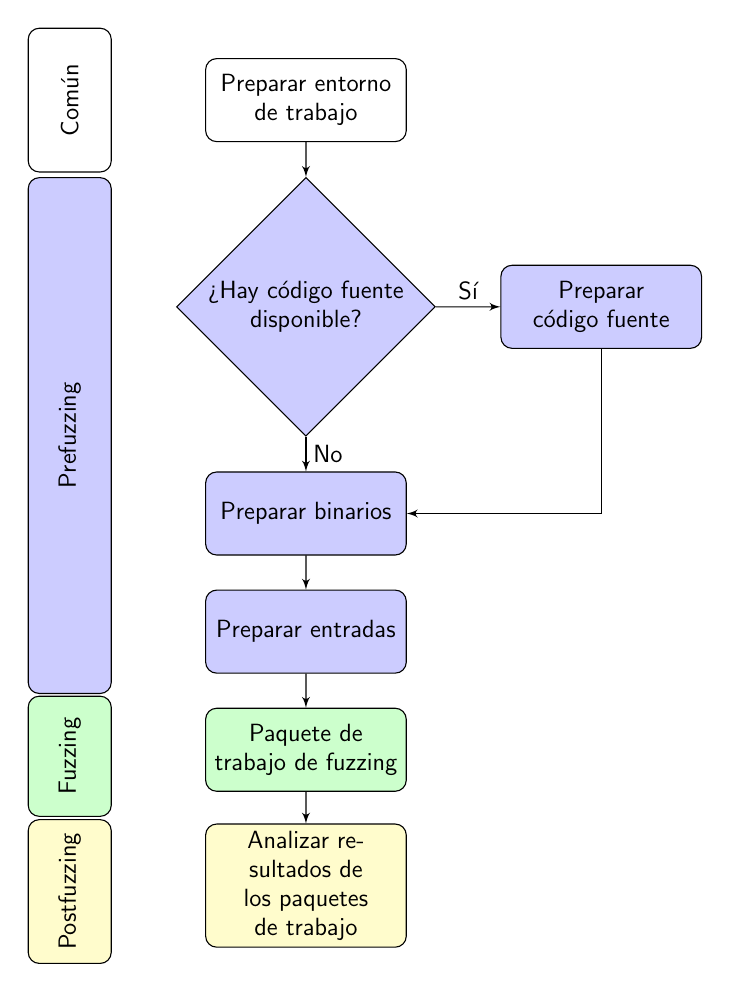
\begin{tikzpicture}[node distance = 2cm, auto,
  % En un paper, las figuras suelen tener una fuente de tipo sin serifa (para
  % distinguirlas del texto). Además, todos elementos de texto deberían tener
  % el mismo tamaño de fuente)
  font=\large\sffamily,
  % Estas dos opciones de tikzpicture son para poder reescalar la imagen
  transform shape, scale=0.75
  ]
    % nodes
    \node [blockWH] (prep_env) {Preparar entorno de trabajo};
    \node [decisionBL, below of = prep_env, node distance = 3.5cm] (Hay_src) {¿Hay código fuente disponible?};
    \node [blockBL, right of = Hay_src, node distance = 5cm] (prep_src) {Preparar código fuente};
    \node [blockBL, below of = Hay_src, node distance = 3.5cm] (prep_bin) {Preparar binarios};
    \node [blockBL, below of = prep_bin, node distance = 2cm] (prep_in) {Preparar entradas};
    \node [blockGR, below of = prep_in, node distance = 2cm] (pruebas) {Paquete de trabajo de fuzzing};
    \node [blockYL, below of = pruebas, node distance = 2.3cm] (resultados) {Analizar resultados de los paquetes de trabajo};

    % edges
    \path [line] (prep_env) -- (Hay_src);
    \path [line] (Hay_src) -- node[midway,above] {Sí} (prep_src);
    \path [line] (Hay_src) -- node[midway,right] {No}(prep_bin);
    \path [line] (prep_bin) -- (prep_in);
    \path [line] (prep_src) |- (prep_bin);
    \path [line] (prep_in) -- (pruebas);
    \path [line] (pruebas) -- (resultados);

  % Leyenda cuqui
  \node [left of={prep_env},xshift=-2cm,blockWH,rotate=90,text width=2.2cm] (center:Common) {Común};
  \node [left of={prep_bin},xshift=-2cm,yshift=1.32cm,blockBL,rotate=90,text width=8.5cm] (center:Prefuzzing) {Prefuzzing};
  \node [left of={pruebas},xshift=-2cm,yshift=-0.11cm,blockGR,rotate=90,text width=1.8cm] (center:Fuzzing) {Fuzzing};
  \node [left of={resultados},xshift=-2cm,yshift=-0.1cm,blockYL,rotate=90,text width=2.2cm] (center:Postfuzzing) {Postfuzzing};

  %\node [above of={center:Common}] {Phases/Steps};

  \end{tikzpicture}
  \caption{ Diagrama de flujo para describir el funcionamiento de HOUSE según las diferentes fases de fuzzing. }
  \label{fig:HOUSE_flow}
\end{figure}


\begin{enumerate}
    \item \textbf{Común o de preparación del entorno de trabajo}.
    Es la única fase transversal a todo el proceso ya que se suele realizar una única vez, bien en la puesta en marcha de las herramientas necesarias para el {\fz} o bien durante el despliegue inicial del marco de trabajo.
    \item \textbf{\textit{Prefuzzing} o de preparación de las pruebas software}.
    En esta fase se elige el tipo de {\fz} a utilizar en función del grado de acceso y las necesidades de adaptación del código fuente. También admite los requisitos o preferencias del tipo de pruebas e incluso los resultados que se persigan con él. En función del tipo elegido, se preparan los binarios correspondientes: empleando binarios ya compilados o realizando una compilación específica si es necesario.
    En función del binario seleccionado, también se confecciona o valida un conjunto de entradas para esa campaña de {\fz}~\cite{fuzzing_SOA}.
    \item \textbf{\textit{Fuzzing} o de ejecución de las propias pruebas}.
    Fase en la que se somete el software bajo prueba (PUT - \textit{Program Under Test}) al {\fz} utilizando la configuración realizada previamente.
    \item \textbf{\textit{Postfuzzing} o de análisis de resultados y tareas posteriores}.
    En esta última fase, bien si se desea o bien si por volumen de trabajo es necesario automatizar la tarea de análisis de resultados, es posible ejecutar un paquete de trabajo creado expresamente para poner en valor los resultados del {\fz}.
\end{enumerate}

A su vez, dicho proceso trabaja sobre un conjunto de datos organizados en seis módulos, que pueden ser orquestados de manera escalable en un entorno de HPC por medio de cargas de trabajo agrupadas por paquetes:

% Comentado para resumir
%
\begin{figure}[htbp]
   \centering
    \resizebox{0.4\textwidth}{!}{\includesvg{./figures/data/Infografia_CASA_paper.svg}} 
    \caption{Infografía módulos marco de trabajo HOUSE.}
    \label{fig:infografia_modulos}
\end{figure}

   

\begin{enumerate}
\item \textbf{\textit{TooL Box} (0.TLB)}.
    Colección de herramientas y utilidades auxiliares a cualquiera de las fases del {\fz}.

\item \textbf{\textit{Source Code Integration} (1.SCI)}.
    Colección de códigos fuente, incluyendo parches, integraciones y optimizaciones previas al {\fz}.
\item \textbf{\textit{Binaries Ready to Fuzz} (2.BRF)}.
    Colección de binarios preparada para el {\fz}.
\item \textbf{\textit{WorkLoad Package} (3.WLP)}.
    Colección de paquetes con cargas de trabajo\footnote{\textbf{Carga de trabajo}~\cite{IEEE_SW_standar}: Combinación de tareas que se ejecutan en un sistema informático determinado. Sus principales características es incluir los requisitos de entrada y salida, cantidad, tipo de calculo y computo requerido.}, que pueden ser de cualquier fase del {\fz}, como herramientas que analicen el código fuente para identificar áreas más propensas a fallos, tareas propias de {\fz} o de analítica de resultados.
\item \textbf{\textit{Input Repository }(A.IR)}.
    Repositorio de entradas como semillas para generadores de entradas, diccionarios, archivos de muestra, etc.
\item \textbf{\textit{Output Repository }(B.OR)}.
    Repositorio de salidas con los contextos de ejecuciones de los \textit{fuzzers}, resultados y cualquier información útil generada por el flujo de trabajo como logs.
\end{enumerate} 
 
Cabe señalar que cada módulo puede estar formado por componentes, unidades funcionales o una combinación de ambos. La principal diferencia entre dichos elementos radica en que las unidades funcionales realizan tareas de automatización o ejecución y los componentes son solo información.
Por otro lado, los módulos identificados por letras (como \textbf{A.IR} y \textbf{B.OR}) están formados únicamente por datos, mientras que los identificados por números (\textbf{0.TLB}, \textbf{1.SCI}, \textbf{2.BRF} y \textbf{3.WLP}) tienen al menos una actividad que forma parte del flujo de {\fz}. En relación a estos últimos, el propio número indica su grado de dependencia dentro del proceso del {\fz}; siendo 0 la más baja y 3 la más alta.

Teniendo en cuenta todo lo anterior,
esta estructura de fases junto a su modularización hacen que HOUSE promueva la reutilización de las diferentes partes del proceso de {\fz}; permitiendo así su escalabilidad o paralelización. Adicionalmente, dicha estructura también permite que el marco de trabajo sea agnóstico a las herramientas {\fz} empleadas. Por ejemplo, es posible cambiar el \textit{fuzzer} utilizado sin tener que rehacer las correspondientes adaptaciones del código fuente, sin tener que preparar nuevos binarios o, incluso, sin tener que parar los trabajos en curso. De igual modo, también permite la reutilización de los conjuntos de datos de entrada creados para un proyecto concreto o el hecho de combinarlos con herramientas que los generen desde archivos de muestra.

\subsection{Flujo de trabajo y procesos asociados}
\label{Flujo_trabajo-procesos}

La Fig.~\ref{fig:tabla_procesos} representa el flujo de trabajo de HOUSE utilizando el lenguaje de modelado \textit{Business Process Model and Notation} (BPMN) en su versión 2.0.2~\cite{BPMN_spec}. La utilización de BPMN responde a la necesidad de modelar de extremo a extremo todo el flujo de {\fz} al detalle suficiente. De haber utilizado el lenguaje UML \textit{(Unified Modeling Language)}, el resultado hubiese sido menos preciso y más complejo al tener menos objetos representables y estar centrado en los flujos de datos.

%%% POSTER FLUJO BAJO NIVEL %%%
\begin{figure*}[p!]
%%\begin{figure*}[ht!]
%%https://www.overleaf.com/learn/latex/Positioning_of_Figures
    \centerline{
    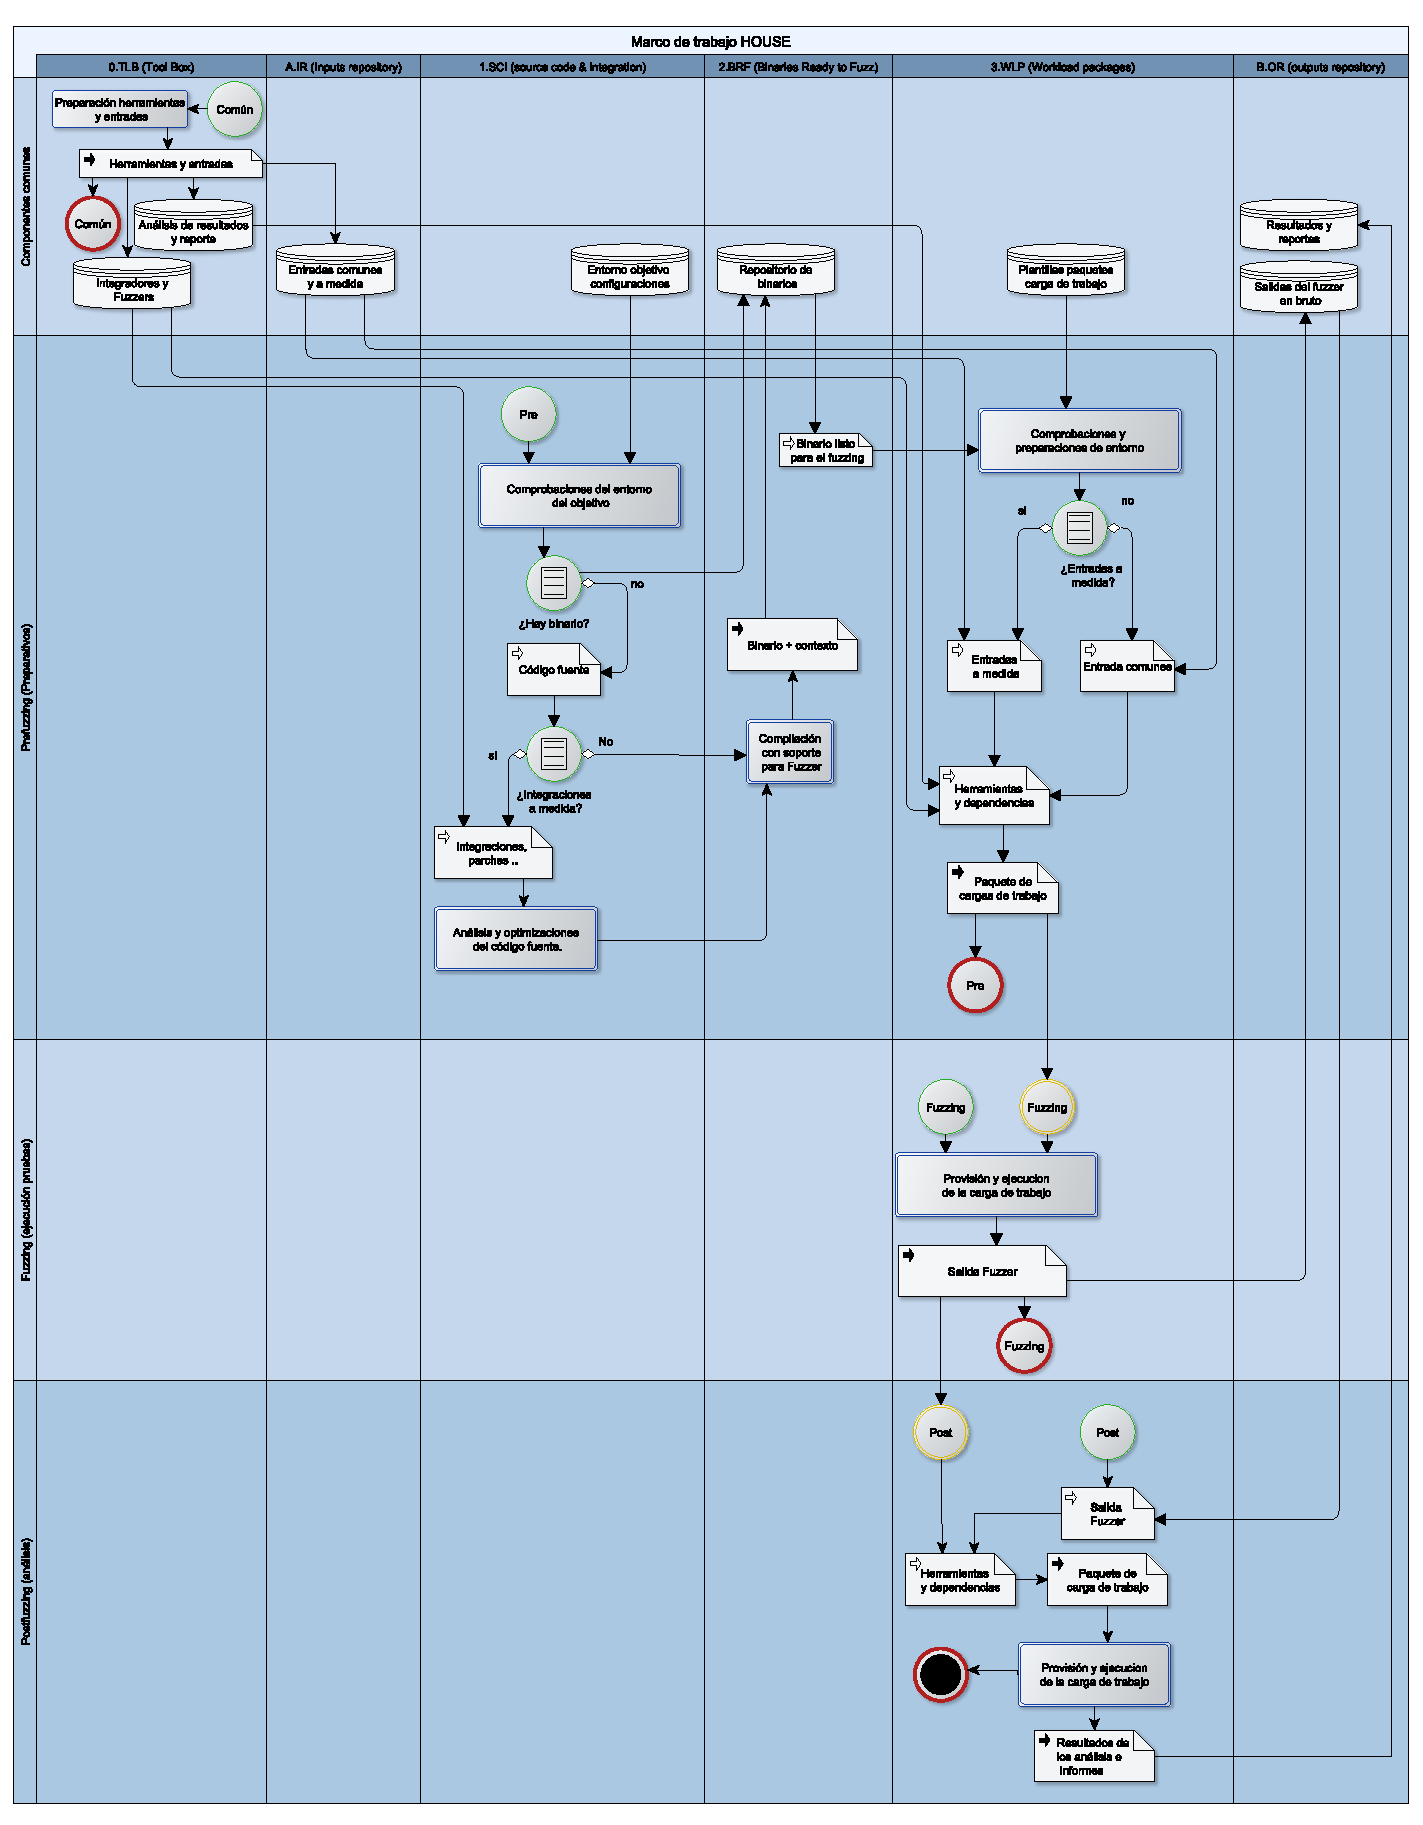
\includegraphics[width=\linewidth]{./figures/data/Tabla_procesos_v5_ES.pdf}    }
    \caption{Diagrama BPMN del marco de trabajo HOUSE.}
    \label{fig:tabla_procesos}
\end{figure*}

   

Dicho lo anterior,
en las columnas del diagrama BPMN de la Fig.~\ref{fig:tabla_procesos} se sitúan los módulos de HOUSE y en las filas sus fases. Los siguientes apartados detallan individualmente esas fases dentro de cada módulo del marco de trabajo.

%====================================================================
\subsubsection{Común}
\label{Fase_comun}

Esta fase aporta el esqueleto necesario para modelar el proceso de {\fz} dentro del marco de trabajo HOUSE. También define los elementos esenciales para las propias tareas de {\fz} o las adyacentes (como por ejemplo los analizadores de código, los generadores de entradas o el reporte de resultados). Dicho de otra manera, esta fase es responsable de habilitar---entre otros elementos---cualquier herramienta, librería o conjunto de datos de entradas que se vayan a utilizar en el entorno de ejecución de las pruebas.
Todo esto se realiza tanto en el módulo \textbf{0.TLB} (para el caso de herramientas tales como \textit{fuzzers}, analizadores u optimizadores de código fuente, generadores de conjuntos de datos de entrada, etc) como en el módulo \textbf{A.IR} (para los diccionarios, muestras de ficheros o conjuntos de datos utilizados).

% Comentado para resumir
%Es necesario recordar que, gracias a la arquitectura de HOUSE, es posible adaptar o integrar nuevas herramientas, colecciones de datos y automatizaciones de una forma común; en lugar de hacerlo de forma específica y concurrente por cada proyecto de {\fz}.

%====================================================================
\subsubsection{\textit{Prefuzzing}}
\label{Fase_prefuzzing}

Todas aquellas tareas previas al {\fz} tales como preparativos, configuraciones, provisiones de muestras o conjuntos de datos forman parte de esta fase. Según el tipo de {\fz} a realizar, las tareas pueden comenzar en el módulo \textbf{1.SCI} o en el \textbf{2.BRF}.

Por un lado, el primer caso se da cuando el tipo de {\fz} seleccionado es \textit{white-box} o \textit{grey-box}; en función de la dependencia de las pruebas del código fuente. En este caso, el módulo es el encargado de realizar las diferentes actividades necesarias para preparar el código fuente de cara a su compilación y atendiendo a las necesidades de alcance, estrategia, requisitos y herramientas elegidas para ese flujo. Por otro lado, el segundo caso se da cuando el tipo de {\fz} seleccionado es \textit{black-box} y, en cuyo caso, el módulo \textbf{1.SCI} no está implicado. Usándose directamente el módulo \textbf{2.BRF}.

Así mismo, el módulo \textbf{2.BRF} es común a cualquier flujo de {\fz} independientemente del tipo empleado. La finalidad de este módulo es realizar el almacenamiento del binario objetivo del {\fz} y el código utilizado para su generación si está disponible; llevando a cabo la compilación del código fuente previamente adecuado dentro del módulo \textbf{1.SCI}. Más aún, en el módulo \textbf{2.BRF} se realizan, si procede, las comprobaciones necesarias para verificar que los binarios son funcionales y también la alineación con la estrategia y requisitos planteados.

Cabe señalar que un punto común entre los módulos \textbf{1.SCI} y \textbf{2.BRF} es el código fuente utilizado en alguno de los tipos de {\fz}. No obstante, existe una diferencia fundamental entre ambos y es el contexto y la finalidad de este último. En el caso de \textbf{1.SCI}, el objetivo es trabajar con el código fuente original del software y realizar las transformaciones necesarias para el {\fz}. Por su parte, en el caso de \textbf{2.BRF} se utiliza un código modificado para un contexto específico de {\fz}. Al mismo tiempo, a nivel de almacenamiento también hay diferencias. Mientras que en \textbf{1.SCI} se asume que el código fuente es una única dependencia asociada a una versión de software, \textbf{2.BRF} mantiene un repositorio con el código modificado y los binarios asociados a este.

También se debe agregar que en esta fase se confecciona el paquete de trabajo para el {\fz} o para cualquier tarea de análisis o generación de dependencias para este, en el módulo \textbf{3.WLP}; en función del tipo de herramienta, técnica empleada y entorno de ejecución de las pruebas. Si es necesario, también se alinean los conjuntos de datos del repositorio \textbf{A.IR}.

Otros posibles usos de los paquetes de trabajo con el fin de ejecutar las tareas de forma escalable o paralelizable son: Los de análisis de código estático para preparar la estrategia de {\fz}, el filtrado de resultados y el uso de generadores de entradas.

% Comentado para resumir
%Por último, una posible tarea que se realiza en esta fase sería la adaptación del código fuente para facilitar las entradas desde ficheros o la entrada estándar de consola. Esto se daría en aquellos casos que se quiera realizar {\fz} de software que utilice comunicaciones de red. De forma similar, otra posible tarea sería el uso de analizadores de código estático para detectar posibles bucles de cara a preparar una adaptación o exclusión o de cara a identificar zonas calientes donde poner el foco.
%%%%%%%%%%%%%%%%%%%%%%%%%%%%%%%%%%%%%%%%%%%%%%%%%%%%%%%%%%%%%%%%%%%%%

%====================================================================
\subsubsection{{\fz}}
\label{Fase_fuzzing}

Esta fase, común a todos los tipos de {\fz}, comprende únicamente el módulo \textbf{3.WLP}. En ella se realizan las tareas de provisión del paquete de trabajo, el seguimiento de su ejecución y el volcado de los resultados en el repositorio de datos de salida en crudo \textbf{{B.OR}}. Un ejemplo de tarea realizada en esta fase dentro del componente \textbf{3.WLP} sería la gestión de colas de trabajo asociadas a un paquete.

%====================================================================
\subsubsection{\textit{Postfuzzing}}
\label{Fase_postfuzzing}

Esta última fase se realiza en el módulo \textbf{3.WLP}. Se centra en el procesamiento y análisis de los resultados de los paquetes de trabajo previos de {\fz}; ultimando para ello el repositorio \textbf{B.OR}. Ejemplos de tareas pertenecientes a esta fase podrían ser el uso de herramientas de filtrado de falsos positivos, la generación de reportes, etc.

%--------------------------------------------------------------------

\section{Prueba de Concepto}
\label{Prueba_de_concepto}

El marco de trabajo HOUSE es \textit{open source} y está disponible públicamente en GitHub~\cite{HOUSE_ref-github_repo}. De cara a validar su propuesta, se está llevando a cabo una prueba de concepto en el entorno de ejecución del HPC Caléndula~\cite{HPC_Leon}. Este entorno utiliza Slurm~\cite{HPC_tool_slurm} como sistema de gestión de cargas y las arquitecturas Intel, Cascade Lake y Haswell, sobre el sistema operativo CentOS 7.7. Calendula cumple con las políticas y requisitos del Esquema nacional de seguridad~\cite{ens_ref-boe}.

Cabe destacar que para la prueba de concepto no se ha utilizado ningún sistema de contenedores en ninguno de los módulos, ni se aplican excepción de políticas de seguridad o uso de permisos especiales.

La prueba de concepto consiste en desarrollar diversos scripts para Slurm e implementar casos de uso básicos con el \textit{fuzzer} AFL++~\cite{fuzz_tool_afl++}, un proyecto \textit{open source} que integra las ultimas técnicas de {\fz} y continúa el proyecto discontinuado de AFL. El tipo de {\fz} elegido para esta prueba fue el \textit{white-box}, utilizando la cobertura de código sobre los binarios \texttt{date} y \texttt{expr} de la colección de utilidades coreutils, perteneciente a los sistemas GNU~\cite{sut_coreutils}. También se incluyó un caso básico de Buffer Overflow. En relación a la entrada de datos, en ambos casos se utilizó la entrada estándar.

Desde el inicio de las actividades se han resuelto distintos problemas derivados de la naturaleza del HPC Calendula, un entorno multipropósito y multiusuario con requisitos de seguridad y privacidad elevados que condicionan el desarrollo.

Los principales problemas identificados son el uso de nodos compartidos, lo que imposibilita relajar las protecciones y mecanismo de monitorización existentes. Destacan las limitaciones de uso de herramientas basadas en ASAN~\cite{ASAN_ref-paper} o la monitorización de \textit{crashes} usando ABRT~\cite{abrt_doc-redhat}, ya sea para evitar bloquear recursos comunes de los nodos o por su uso como parte de las protecciones de los sistemas. Esto se soluciona utilizando otras estrategias de detección basadas totalmente en instrumentación.

Inicialmente se trató de evitar complejidad usando la instrumentación mas básica del AFL++, afl-gcc similar a la del experimento, para reducir el número de dependencias y la complejidad para la prueba de concepto. Por los problemas anteriormente mencionados, se está trabajando en la adecuación de instrumentación apoyada en LLVM.

%%%%%%%%%%%%%%%%%%%%%%%%%%%%%%%%%%%%%%%%%%%%%%%%%%%%%%%%%%%%%%%%%%%%%

\begin{figure}[htbp]
     \centering
    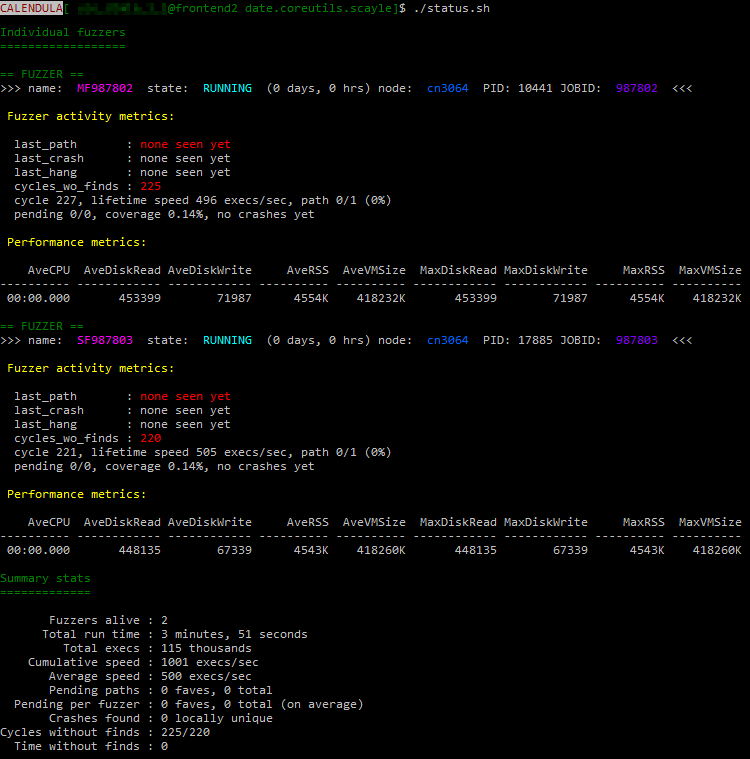
\includegraphics[width=0.5\textwidth]{./figures/data/Image_fuzzer_status_HOUSE.png}
    \caption{Ilustración status de los trabajos de fuzzing.}
    \label{img:fuzzer_status}
\end{figure}


En la Fig.~\ref{img:fuzzer_status} se puede observar la ejecución de un paquete de trabajo de {\fz} utilizando dos trabajos y las métricas de rendimiento y actividad. Así como el sumatorio total de la actividad de todos los \textit{fuzzers}.

%--------------------------------------------------------------------
\section{Conclusiones}
\label{Conclusiones}

%%% Resumen con foco en los resultados.
El {\fz} está cobrando cada vez más protagonismo como actividad para garantizar la calidad y la seguridad del software. Esta tendencia es utilizada por empresas y organizaciones para poner en valor sus desarrollos o servicios de forma comercial, a la vez que anima al desarrollo de mejoras y herramientas. Esta situación provoca la dependencia tecnológica y un riesgo a la confidencialidad para su adopción en un ciclo de desarrollo seguro y dificulta la puesta en marcha. Esta dependencia también frena la adopción de mejoras, el uso de alternativas totalmente libres y agnósticas de la tecnología.

HOUSE propone un modelado del flujo de trabajo del {\fz} caracterizado por tener un enfoque abierto y agnóstico a las herramientas. Con esta finalidad, el marco de trabajo propone una visión ordenada de todas las fases previas y posteriores a las pruebas. De esta manera, HOUSE permite resolver o simplificar las tareas más tediosas y complejas relacionadas con la aplicación de técnicas de {\fz}.

Este flujo se basa en los pasos y elementos establecidos en la Fig.~\ref{fig:tabla_procesos}.

%%% "Conclusion resultados"

%No hay ningún enfoque de fuente abierta que abarque todas las fases del {\fz} como un único flujo con una orientación modular que permita a los desarrolladores e investigadores minimizar la barrera de entrada o una integración sencilla.

%Solo se ha identificado un experimento en un entornos de supercomputación real~\cite{HPC_fuzzing}, sin acceso a los desarrollo implicados y basado en herramientas discontinuadas.

% Párrafo movido de más arriba
Así pues, esta investigación sienta las bases teóricas comunes y las prácticas mínimas de un marco de trabajo que permite reducir el esfuerzo inicial a la hora de poner en marcha un entorno de {\fz} escalable que garantice la confidencialidad de la información. De igual modo, HOUSE facilita, tanto a investigadores como a desarrolladores, el hecho de poder trabajar en un componente o funcionalidad específica o el hecho de incluir aquellas características de seguridad proactiva en el software dentro de su ciclo de desarrollo. Estos aspectos se traducen en una reducción de la carga de trabajo en tareas auxiliares o distintas a las de los objetivos planificados.

Esta primera versión del marco de trabajo brinda la estructura de directorios, repositorios de datos y recursos para utilizar el AFL++~\cite{fuzz_tool_afl++} con instrumentación básica, incluyendo las automatizaciones para la creación de cargas de trabajo, usando un sistema de colas Slurm~\cite{HPC_tool_slurm}. 


%--------------------------------------------------------------------

\section*{Agradecimientos}

%\begin{itemize}
%\item \href{https://www.scayle.es/}{\textbf{SCAYLE}}, centro de supercomputación de la Junta de Castilla y León.
%\item \href{https://robotica.unileon.es}{Grupo de Robótica} de la Universidad de León. 
%\end{itemize}

Este trabajo ha sido parcialmente financiado por INCIBE mediante la Adenda 4 al convenio marco con la Universidad de León. Los autores agradecen al centro de supercomputación SCAYLE la posibilidad de utilizar sus infraestructuras para validar la propuesta presentada en este trabajo de investigación.

%--------------------------------------------------------------------

%%% BIBLIOGRAFÍA %%%
\bibliographystyle{IEEEtran}
\bibliography{bibliography}

\end{document}
